\fancyhead[LE,RO]{\textbf{\textsf{26}}}
\fancyhead[RE]{\textbf{\textsf{CHƯƠNG 1}}\quad \textsf{Hàm số và Mô hình}}
\fancyhead[LO]{}

\noindent
\begin{minipage}[t]{0.26\textwidth}
    \vspace{0pt}
    \raggedright
    \vspace{6.15cm} % Căn chỉnh vị trí Bảng 2 tương ứng ngang hàng với Ví dụ 4
    
    \textbf{\textsf{Bảng 2}}
    \vspace{1mm}
    
    \renewcommand{\arraystretch}{1.15}
    \begin{tabular}{|c|c|}
        \hline
        \rowcolor{stewartcyan!20}
        \parbox{1.5cm}{\centering \textsf{\textbf{Thời gian}}\\\textsf{(giây)}} & \parbox{1.5cm}{\centering \textsf{\textbf{Độ cao}}\\\textsf{(mét)}} \\
        \hline
        0 & 450 \\
        1 & 445 \\
        2 & 431 \\
        3 & 408 \\
        4 & 375 \\
        5 & 332 \\
        6 & 279 \\
        7 & 216 \\
        8 & 143 \\
        9 & 61 \\
        \hline
    \end{tabular}

    \vspace{3.44cm}
    
    \textbf{\textsf{HÌNH 9}}\\[1mm]
    \textsf{Biểu đồ phân tán cho quả bóng rơi}
    
\end{minipage}%
\hfill
\begin{minipage}[t]{0.71\textwidth}
    \vspace{0pt}
    và được gọi là một \textbf{hàm bậc ba} (\textit{cubic function}). \textbf{\textsf{Hình 8}} thể hiện đồ thị của một hàm bậc ba ở phần (a) và đồ thị của các đa thức bậc 4 và bậc 5 ở các phần (b) và (c). Sau này chúng ta sẽ thấy lý do tại sao các đồ thị lại có những hình dạng này.

    \vspace{3mm}
    \noindent
    \begin{minipage}[b]{0.16\textwidth}
        \textbf{\textsf{HÌNH 8}}
    \end{minipage}%
    \begin{minipage}[b]{0.28\textwidth}
        \centering
        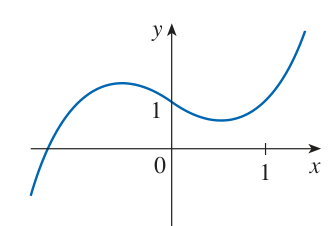
\includegraphics[width=\textwidth]{images/p0061_fig1.png}\\
        \vspace{1mm}
        {\footnotesize (a) $y = x^3 - x + 1$}
    \end{minipage}\hfill
    \begin{minipage}[b]{0.28\textwidth}
        \centering
        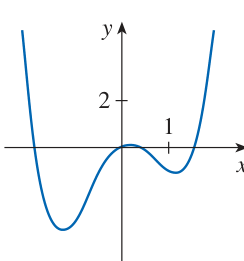
\includegraphics[width=\textwidth]{images/p0061_fig2.png}\\
        \vspace{1mm}
        {\footnotesize (b) $y = x^4 - 3x^2 + x$}
    \end{minipage}\hfill
    \begin{minipage}[b]{0.28\textwidth}
        \centering
        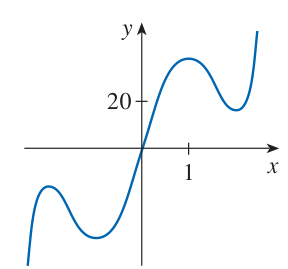
\includegraphics[width=\textwidth]{images/p0061_fig3.png}\\
        \vspace{1mm}
        {\footnotesize (c) $y = 3x^5 - 25x^3 + 60x$}
    \end{minipage}

    \vspace{4mm}
    Các hàm đa thức thường được sử dụng để mô hình hóa các đại lượng khác nhau xuất hiện trong khoa học tự nhiên và khoa học xã hội. Chẳng hạn, trong \textbf{\textsf{Mục 3.7}} chúng ta sẽ giải thích tại sao các nhà kinh tế học thường sử dụng một hàm đa thức $P(x)$ để đại diện cho chi phí sản xuất $x$ đơn vị hàng hóa. Trong ví dụ sau đây, chúng ta sử dụng một hàm bậc hai để mô hình hóa sự rơi của một quả bóng.

    \vspace{3mm}
    \noindent\textbf{\textsf{\color{stewartcyan}VÍ DỤ 4}}\quad Một quả bóng được thả rơi từ đài quan sát trên cao của Tháp CN, cách mặt đất $450\text{ m}$, và độ cao $h$ của nó so với mặt đất được ghi lại sau mỗi khoảng thời gian 1 giây trong Bảng 2. Hãy tìm một mô hình phù hợp với dữ liệu và sử dụng mô hình đó để dự đoán thời điểm quả bóng chạm đất.

    \vspace{2mm}
    \noindent\textbf{\textsf{\color{stewartcyan}LỜI GIẢI}}\quad Chúng ta vẽ biểu đồ phân tán của dữ liệu trong Hình 9 và nhận thấy rằng một mô hình tuyến tính là không phù hợp. Tuy nhiên, các điểm dữ liệu trông có vẻ như nằm trên một parabol, vì vậy chúng ta thử dùng một mô hình bậc hai thay thế. Sử dụng máy tính cầm tay có chức năng vẽ đồ thị hoặc hệ thống đại số máy tính (vốn sử dụng phương pháp bình phương bé nhất), ta thu được mô hình bậc hai sau:
    \begin{equation}
        \llap{\fcolorbox{stewartred}{white}{\textcolor{stewartred}{\textbf{3}}}\qquad}
        h = 449.36 + 0.96t - 4.90t^2
    \end{equation}

    \vspace{1mm}
    \noindent
    \begin{minipage}[t]{0.48\textwidth}
        \centering
        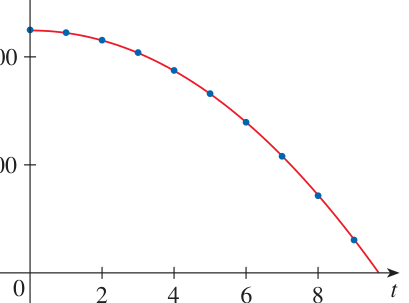
\includegraphics[width=\textwidth]{images/p0061_fig4.png}
    \end{minipage}\hfill
    \begin{minipage}[t]{0.48\textwidth}
        \centering
        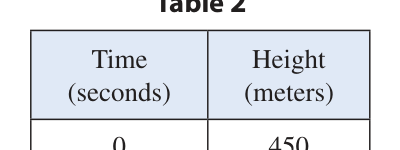
\includegraphics[width=\textwidth]{images/p0061_fig5.png}
        \vspace{2mm}
        \raggedright
        \textbf{\textsf{HÌNH 10}}\\[1mm]
        \textsf{Mô hình bậc hai cho quả bóng rơi}
    \end{minipage}

    \vspace{4mm}
    Trong Hình 10, chúng ta vẽ đồ thị của Phương trình 3 cùng với các điểm dữ liệu và nhận thấy rằng mô hình bậc hai cho kết quả khớp rất tốt.

    Quả bóng chạm đất khi $h = 0$, do đó chúng ta giải phương trình bậc hai:
    \[
    -4.90t^2 + 0.96t + 449.36 = 0
    \]
\end{minipage}